% ==============================================================================
% 插曲 4：数的本质 (Intermezzo 4: The Nature of Numbers)
% ==============================================================================

\intermezzo{插曲 4：数的本质}
\label{sec:intermezzo04}

当谈及“数”时，程序设计语言充当了底层物理硬件与纯粹数学之间的调解者。典型的计算机硬件是用固定大小的内存块（位 bit、字节 byte、字长 word）来表示数据的；其处理器也是专门针对这些定长数据块来设计计算指令的。

在纸笔演算的纯粹数学中，我们从不需要担心能处理多少位数字——原则上，无论一个数包含 1 位、10 位还是 10,000 位数字，数学运算法则都毫无二致。如果一门编程语言直接采用底层硬件支持的定长数值，其计算效率自然最高；但如果它完全遵循纯数学的精确数值定义，就必须在任意精度数学表示与定长硬件数据块之间频繁转换，而这种转换伴随着时间与空间开销。绝大多数通用编程语言为了极致的执行效率，都妥协选择了基于硬件的定长数值方案。

本篇插曲将深入剖析计算机中定长数表示的本质机制。我们将定义一套定长数的数据表示，探讨其运算实现，并揭示由此带来的两大经典数学困境：\term{算术溢出}（overflow）与\term{算术下溢}（underflow）。最后，我们将展示浮点数在实际计算中可能引发的灾难性精度丢失与混乱现象。

\intermezzosection{定长数运算 (Fixed-Size Number Arithmetic)}
\label{sec:int4_fixed_size}

假设我们只能使用 4 位十进制数字来表示数。如果要表示自然数，其范围为 $[0, 10000)$。如果要表示实数，我们可以在 $[0, 1)$ 区间内均匀选取 10,000 个小数，或者在 $[0, 1)$ 区间选 5,000 个、在 $[1, 2)$ 区间选 5,000 个。无论如何划分，4 位数字最多只能表示 10,000 个离散的数值，而数学连续轴上的实数却有无穷多个。

硬件通用的解决方案是采用\term{科学记数法}（scientific notation）。一个数由两部分组成：
\begin{enumerate}
  \item \term{尾数}（mantissa，记为 $m$）：基准有效数字；
  \item \term{指数}（exponent，记为 $e$）：确定以 10 为底的放大或缩小倍数。
\end{enumerate}

其数学公式表示为：
\[
n = m \times 10^e
\]
例如，数值 1200 可以表示为 $12 \times 10^2$ 或 $120 \times 10^1$。

通过引入符号位，指数可以取负数，从而表示微小的小数：
\[
m \times 10^{-e} = \frac{m}{10^e}
\]

为了在我们的 4 位模型中实现该方案，我们分配 2 位用于尾数、2 位用于指数，外加 1 位指数符号位。据此：
\begin{itemize}
  \item 零表示为：$0 \times 10^0$；
  \item 最大正数为：$99 \times 10^{99}$（99 后面紧跟 99 个零）；
  \item 最小正小数为：$1 \times 10^{-99}$。
\end{itemize}

我们在 ISL+ 中为定长科学记数法建立如下数据定义：

\begin{lstlisting}[language=BSL]
(define-struct inex [mantissa sign exponent])

; 一个 Inex 是一个结构体：
;   (make-inex N99 S N99)

; 一个 S 是下列之一：
; -- 1
; -- -1

; 一个 N99 是介于 0 到 99 之间的整数（含两端边界）。
\end{lstlisting}

图~\ref{fig:143} 给出了安全构建器 \code{create-inex} 与数值还原函数 \code{inex->number}。

\begin{figure}[htbp]
  \centering
  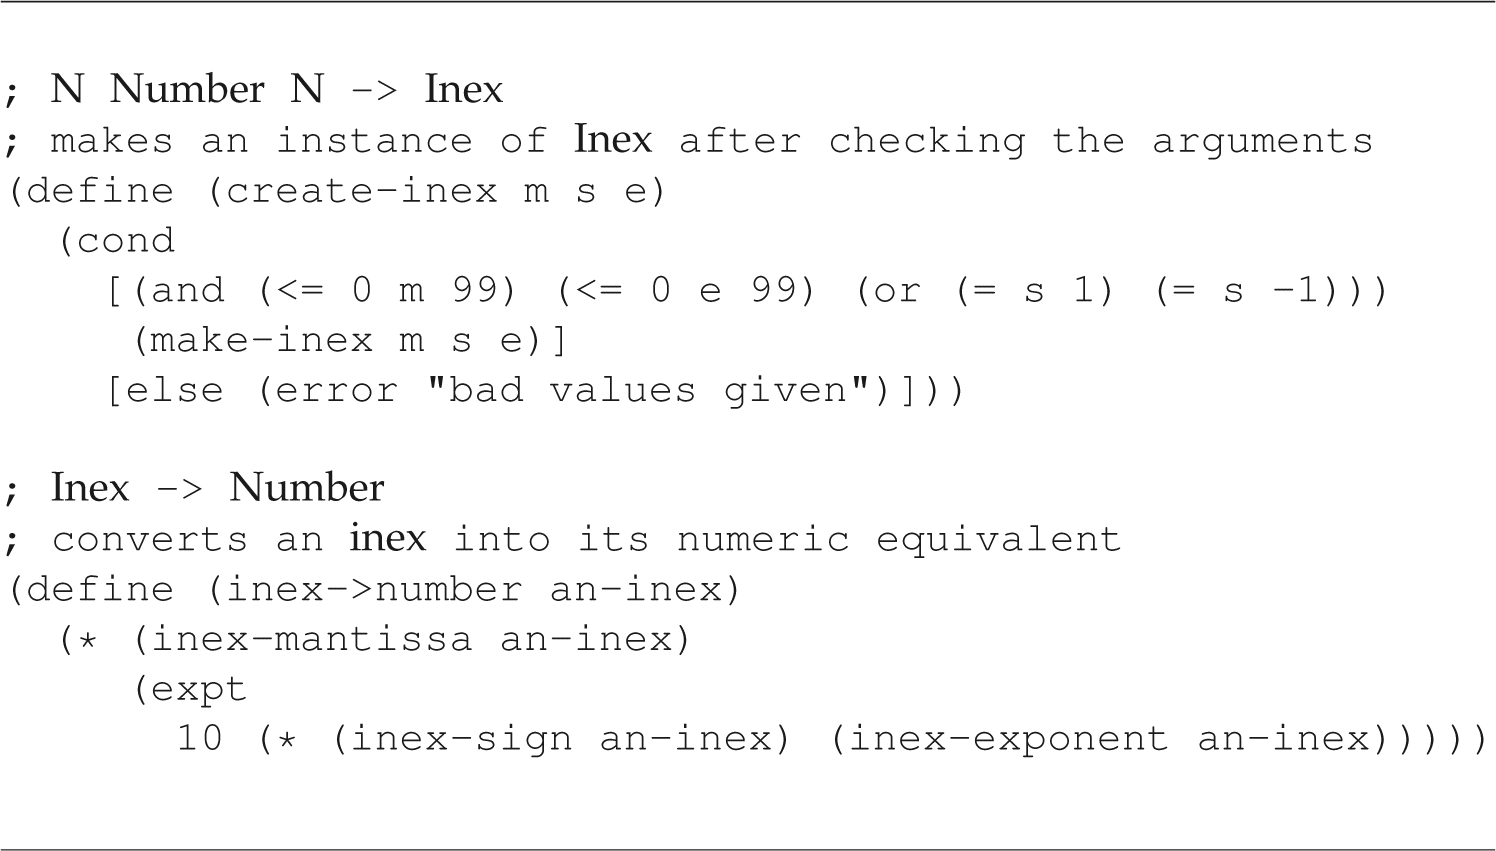
\includegraphics[width=0.85\textwidth]{images/00565.png}
  \caption{不精确数表示与转换函数 (Functions for inexact representations)}
  \label{fig:143}
\end{figure}

借助这一表示，我们可以明确界定可表示数字的范围：
\begin{lstlisting}[language=BSL]
(define MAX-POSITIVE (create-inex 99 1 99))
(define MIN-POSITIVE (create-inex 1 -1 99))
\end{lstlisting}

任何大于 \code{MAX-POSITIVE} 的正数，或者介于 0 与 \code{MIN-POSITIVE} 之间的微小正数，都\textbf{无法在该系统中找到等价表示}。此外，该表示在数轴中间存在巨大的“间隙”：例如 \code{(create-inex 12 1 2)}（即 1200）的下一个紧邻数是 \code{(create-inex 13 1 2)}（即 1300），介于 1200 与 1300 之间的任意数（例如 1240）只能被强行舍入近似到其中之一。这就是计算机科学中所说的\term{不精确数}（inexact numbers）。

\begin{exercise}{设计不精确数加法 inex+}{412}
设计函数 \code{inex+}。该函数实现两个 \code{Inex} 数字的加法运算。当两个输入的指数相同时，只需将尾数相加；当指数不同时，必须先对齐指数。若相加后的尾数超过 99，需进行进位与舍入处理。
\end{exercise}

\begin{exercise}{设计不精确数乘法 inex*}{413}
设计函数 \code{inex*}。该函数计算两个 \code{Inex} 数字的乘积：尾数相乘，指数相加，最后调整规格化并舍入。
\end{exercise}

\begin{exercise}{表示间隙与代数性质的丧失}{414}
由于存在舍入间隙，定长不精确数在数学上往往\textbf{不再满足加法结合律}或\textbf{乘法分配律}！试在你的 \code{Inex} 系统中找出三个数字 $a, b, c$，使得：
\[
(a + b) + c \neq a + (b + c)
\]
\end{exercise}

\intermezzosection{溢出与下溢 (Overflow and Underflow)}
\label{sec:int4_overflow_underflow}

当计算结果超出了系统所能表示的最大限度时，便发生了\term{算术溢出}（arithmetic overflow）。在 ISL+ 中，超出上限的浮点计算结果被标记为特殊值 \code{+inf.0}（表示正无穷大）或 \code{-inf.0}（负无穷大）。

反之，当一个非零计算结果太过于接近零，以至于其量级小于系统能表示的最小正数时，就发生了\term{算术下溢}（arithmetic underflow）。在 ISL+ 中，下溢被粗暴地截断近似为 \code{\#i0.0}。

\begin{exercise}{溢出界限探索}{415}
在 ISL+ 中，找出使得 \code{(expt 10.0 n)} 发生溢出并返回 \code{+inf.0} 的最小正整数 $n$。
\end{exercise}

\begin{exercise}{下溢界限探索}{416}
在 ISL+ 中，找出使得 \code{(expt 10.0 (- n))} 发生下溢并塌缩为 \code{\#i0.0} 的最小正整数 $n$。
\end{exercise}

\begin{exercise}{微指数幂运算精度对比}{417}
在完整 Racket 与 ISL+ 中分别求值表达式：
\begin{lstlisting}[language=BSL]
(expt 1.001 1e-12)
\end{lstlisting}
解释你在两个环境下观察到的输出差异。
\end{exercise}

\begin{exercise}{自定义幂函数 my-expt}{418}
不使用内置的 \code{expt}，针对整数指数设计递归幂函数 \code{my-expt}。在极大与极小测试用例上验证其行为。
\end{exercise}

\intermezzosection{灾难性抵消与求和次序 (Catastrophic Cancellation)}
\label{sec:int4_cancellation}

当一个极大的浮点数与一个极小的浮点数相加时，较小数的信息往往在指数对齐时被完全截断抹杀：
\begin{replbox}
> (+ 1e16 1.0 -1e16)
0.0
> (+ 1e16 (- 1e16) 1.0)
1.0
\end{replbox}
仅仅改变了运算的结合与求和次序，计算结果竟然相差了 $100\%$！

图~\ref{fig:144} 展示了一个著名的“双面简努斯”（Janus-faced）交错级数序列：正向累加与反向累加将得出天壤之别的荒谬结果。

\begin{figure}[htbp]
  \centering
  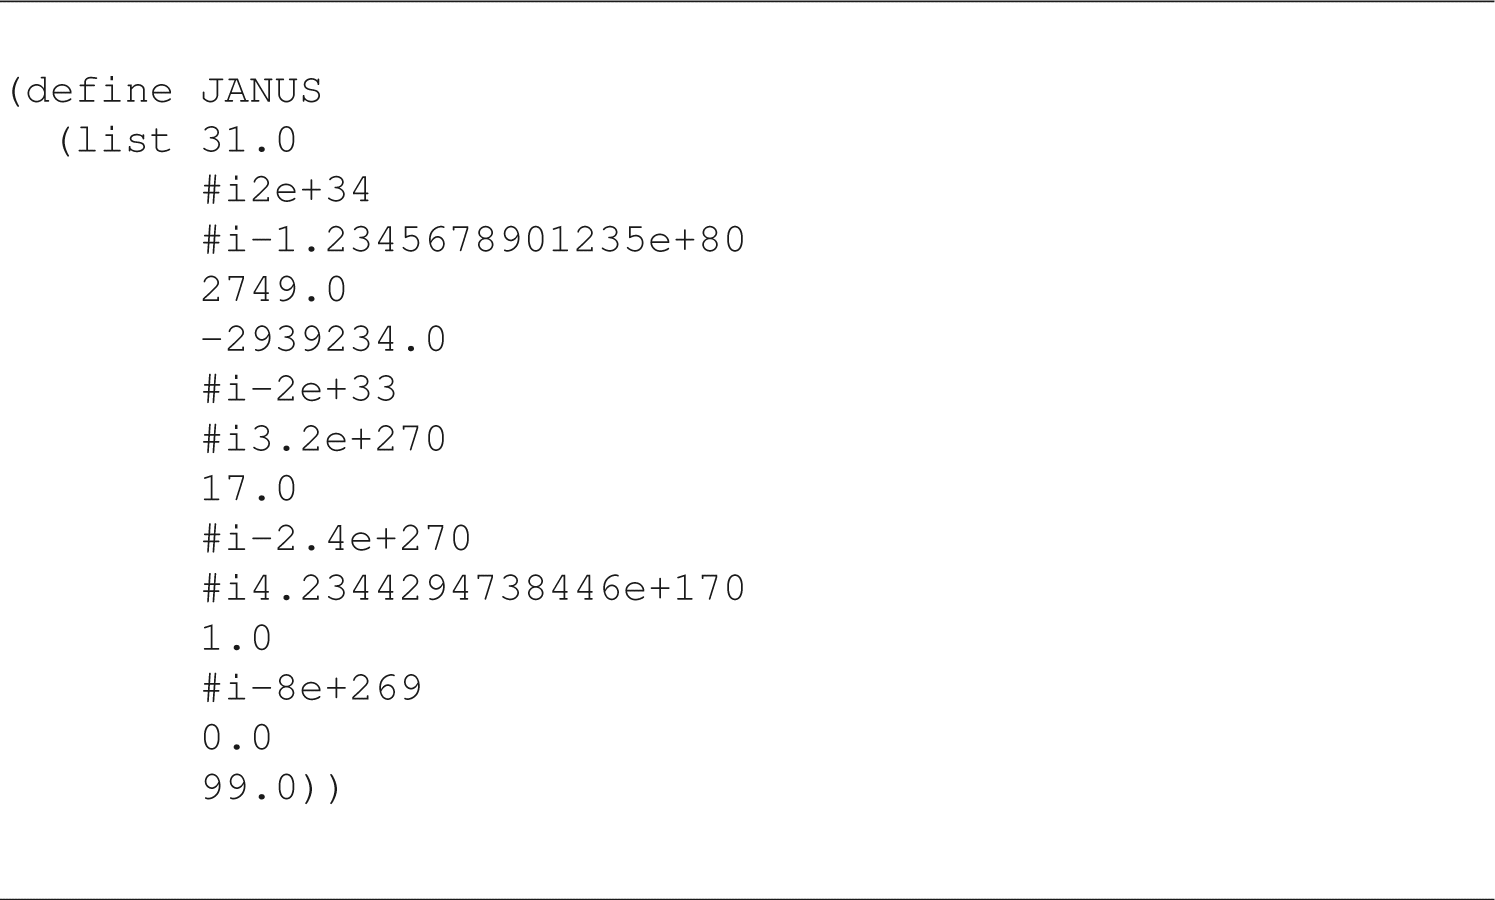
\includegraphics[width=0.85\textwidth]{images/00578.png}
  \caption{双面简努斯不精确数列 (A Janus-faced series of inexact numbers)}
  \label{fig:144}
\end{figure}

\begin{exercise}{求和次序对精度的剧烈影响}{419}
分别使用从左到右正向求和（\code{foldl}）与从右到左反向求和（\code{foldr}）计算图~\ref{fig:144} 中的数列之和。观察并分析两种不同求和方向所带来的致命精度偏差。
\end{exercise}

\begin{exercise}{数值震荡与混沌现象}{420}
考虑如下递归差分方程：
\begin{lstlisting}[language=BSL]
(define (oscillate n)
  (cond
    [(= n 0) 1.0]
    [else (- (* 2 (oscillate (sub1 n))) 1.0)]))
\end{lstlisting}
在纯数学上，$n=0$ 时为 1.0，随后每一项 $2(1.0) - 1.0 = 1.0$，序列应该恒等于 1.0。
然而在计算机浮点运算中，观察该函数随着 $n$ 的增大在图~\ref{fig:145} 中所呈现出的剧烈混沌震荡！
\end{exercise}

\begin{figure}[htbp]
  \centering
  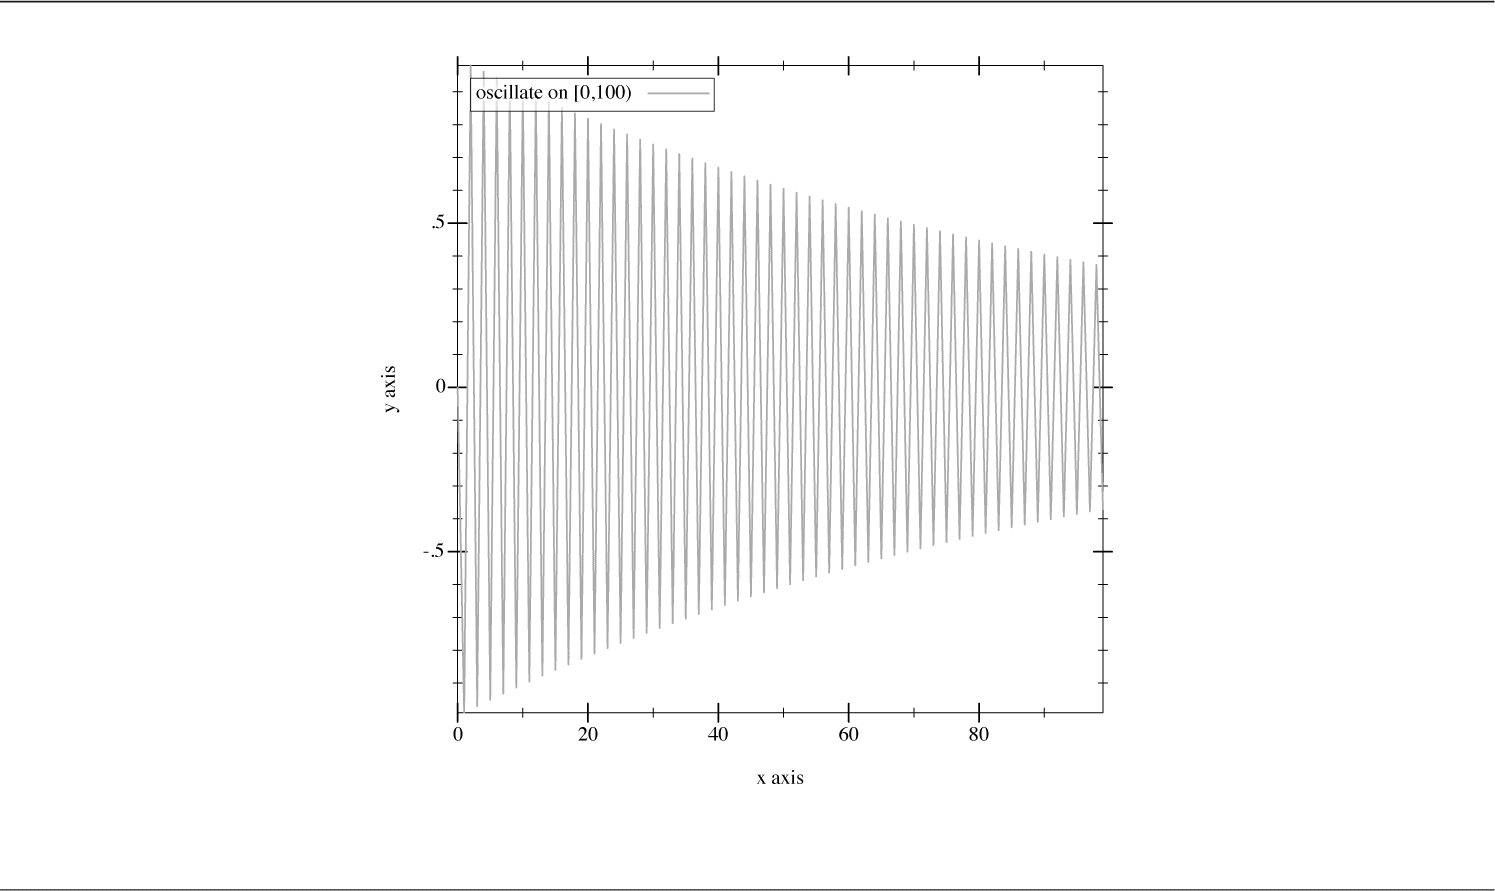
\includegraphics[width=0.85\textwidth]{images/00580.png}
  \caption{数值震荡与浮点混沌 (The graph of oscillate)}
  \label{fig:145}
\end{figure}

\begin{notebox}[结语：敬畏计算中的数字]
计算不仅是纯粹逻辑的演绎，更是物理机器对现实数学的有限逼近。作为优秀的程序设计者，在构建涉及工程、物理模拟与高频金融等涉及实数运算的系统时，必须始终对定长数的精度边界保持高度警惕与敬畏。
\end{notebox}
